%% ===========================================================================
%% A Reproducible Multi-pollutant Railway Emissions Inventory for Pakistan
%% Target journal: Environmental Modelling & Software (Elsevier)
%% ===========================================================================
\documentclass[5p,times,authoryear]{elsarticle}
% ===========================================================================
% Shared preamble for every manuscript in this repository.
%
% Papers using it:
%   paper/            agriculture inventory
%   paper_nowcast/    agricultural nowcasting
%   paper_national/   the nine-sector national inventory
%   notes/<sector>/   one data note per non-agriculture sector
%
% It exists because paper/ and paper_nowcast/ began as copies of one another
% and had already drifted five lines apart before a third manuscript existed.
% Eleven copies would drift eleven ways, and a macro that renders differently
% in two papers is the kind of defect nobody notices until proof stage.
%
% \graphicspath is deliberately NOT set here - each manuscript sets its own
% after \input{...preamble}, because figures live beside the document.
% ===========================================================================

\usepackage[utf8]{inputenc}
\usepackage[T1]{fontenc}
\usepackage{amsmath,amssymb}
\usepackage{graphicx}
\usepackage{booktabs}
\usepackage{multirow}
\usepackage{siunitx}
\usepackage[colorlinks=true,citecolor=blue,linkcolor=blue,urlcolor=blue]{hyperref}
% Document-information metadata for every PDF in the bundle (the seventh review noted
% the shipped PDFs carried none). Documents that set their own \hypersetup{pdftitle=...}
% keep it - hyperref takes the LAST setting, and this shared block runs first. Full
% tagged-PDF (tagpdf / \DocumentMetadata) is deliberately not attempted here: the
% installed LaTeX toolchain's support is not uniform across sixteen documents, and a
% half-tagged bundle is worse than an honestly untagged one; deferred deliberately.
\hypersetup{
  pdfauthor={Rehan Ahmad, Pakistan Air Quality Initiative (PAQI)},
  pdfsubject={A reproducible ten-sector national greenhouse-gas inventory
              for Pakistan},
  pdfkeywords={Pakistan, greenhouse gas inventory, IPCC 2006 Guidelines, MRV,
               reproducible research, emissions, air pollutants},
}
\usepackage{caption}
\captionsetup[table]{position=below}
\usepackage{enumitem}
\usepackage{xcolor}
\usepackage{float}
\usepackage{placeins}
\usepackage{tabularx}
\usepackage{natbib}
\usepackage{tikz}
\usetikzlibrary{arrows.meta,positioning,fit,backgrounds}

\setlength{\emergencystretch}{3em}

% Looser float placement to prevent pile-up in two-column mode.
\renewcommand{\topfraction}{0.95}
\renewcommand{\bottomfraction}{0.85}
\renewcommand{\textfraction}{0.05}
\renewcommand{\floatpagefraction}{0.85}
\setcounter{topnumber}{4}
\setcounter{bottomnumber}{3}
\setcounter{totalnumber}{6}

% ---------------------------------------------------------------------------
% Custom shorthand: in macros.tex since the ESSD re-targeting, because the national
% article compiles under the Copernicus class and cannot take this preamble (the class
% loads its own packages) but needs exactly the same macros. This file inputs it so that
% every other manuscript keeps compiling unchanged.
%
% THREE relative paths, because \input resolves against the COMPILE DIRECTORY and not
% against this file, so the depth is a property of whoever is building:
%   ../paper_common      a manuscript compiled from one level down
%   ../../paper_common   papers/<sector>/ and notes/<sector>/
%   ../../../paper_common  paper_national/versions/<v>/, since the national paper was
%                          versioned - that move is what added this third arm, and the
%                          supplement failed with "../../paper_common/macros.tex not
%                          found" until it was here
% A fourth depth needs a fourth arm, which is the cost of keeping a bare `latexmk` in a
% manuscript directory working without a TEXINPUTS set for it.
% ---------------------------------------------------------------------------
\IfFileExists{../paper_common/macros.tex}%
  {\input{../paper_common/macros}}%
  {\IfFileExists{../../paper_common/macros.tex}%
    {% ===========================================================================
% paper_common/macros.tex - the shorthand every manuscript shares.
%
% Split from preamble.tex in the ESSD re-targeting: the national article now compiles
% under the Copernicus class, which loads its own packages and forbids most of what
% preamble.tex sets (geometry-like options, a second hyperref, placeins), but it needs
% exactly the same shorthand as the sector reports. The macros therefore live here, on
% their own, and preamble.tex inputs this file so that every other manuscript keeps
% compiling unchanged. A macro that renders differently in two documents is the defect
% this file exists to prevent; define it once.
%
% Requires: siunitx (for \DeclareSIUnit and \si) - the caller loads it.
% ===========================================================================

% Gas and pollutant names.
\newcommand{\COtwo}{CO\textsubscript{2}}
\newcommand{\COe}{CO\textsubscript{2}e}
\newcommand{\CHfour}{CH\textsubscript{4}}
\newcommand{\NtwoO}{N\textsubscript{2}O}
\newcommand{\NHthree}{NH\textsubscript{3}}
\newcommand{\NOx}{NO\textsubscript{x}}
\newcommand{\SOtwo}{SO\textsubscript{2}}
\newcommand{\PM}{PM\textsubscript{2.5}}
\newcommand{\MCF}{MCF}
\newcommand{\Mt}{\text{Mt~\COe}}
\newcommand{\tCha}{\si{\tonne\per\hectare}}
\newcommand{\AFOLU}{AFOLU}
\newcommand{\GLW}{GLW\,4}
\newcommand{\EFone}{EF\textsubscript{1}}

% siunitx: allow Mt, Tg, ha, head, yr, dB
\DeclareSIUnit{\head}{head}
\DeclareSIUnit{\yr}{yr}
\DeclareSIUnit{\dB}{dB}

% A file name is the one long unbreakable token these documents are full of -
% \texttt{waste\_air\_pollutants\_2024.csv} is wider than a two-column measure and TeX prints
% it past the margin rather than breaking it. Allowing a break AFTER each escaped underscore
% costs nothing and inserts no hyphen, which matters: a hyphenated file name is a wrong file
% name. This is one line because every such name in every document is written with \_.
\let\pkinvunderscore\_
\renewcommand{\_}{\pkinvunderscore\allowbreak}
}%
    {\input{../../../paper_common/macros}}}
% Long unbreakable strings - output filenames, module paths, URLs in \texttt - do not fit a
% two-column measure and TeX prints them past the margin rather than breaking them. Nothing
% read the log, so 47 of those overruns shipped across seven documents. Emergency stretch lets
% the paragraph loosen instead, and \texttt is taught to break at the punctuation these names
% actually contain.
\emergencystretch=6em


\graphicspath{{figures/}}
\journal{Environmental Modelling \& Software}
\begin{document}
\begin{frontmatter}
\title{PakEmis Sector Technical Note TN09\\[4pt]
A Reproducible Multi-pollutant Railway Emissions Inventory for Pakistan with
Fuel-Balance Closure and Route-Constrained Spatial Allocation}
\author[paqi]{Rehan Ahmad\corref{cor1}}
\ead{rehan@pakairquality.com}
\address[paqi]{Pakistan Air Quality Initiative (PAQI), Karachi, Pakistan}
\cortext[cor1]{Corresponding author}
\begin{abstract}
Pakistan's railway sector has existed in public inventories as a single number---and
officially, a wrong one. This paper presents a complete, reproducible inventory of the
railway module built on the strongest activity datum a sector can have: the operator's own
metered fuel consumption, published annually---\num{132588} thousand litres of diesel in
the FY2023--24 reference year, \SI{0.394}{\mega\tonne} \COe{} in all, of which
\SI{0.389}{\mega\tonne} is strict locomotive traction at IPCC 1A3c and
\SI{0.005}{\mega\tonne} is the measured non-traction claimant, booked at its own
category pending an unresolved 1A2/1A4c end-use split. Around that control it adds
the first railway air-pollutant layer for Pakistan (EMEP/EEA Tier~1:
\SI{5.87}{\kilo\tonne} NO\textsubscript{x}, \SI{0.154}{\kilo\tonne} PM\textsubscript{2.5},
black carbon as the chapter's declared fraction, and \SOtwo{} as an explicit sulfur-case
ladder spanning \SIrange{10}{10000}{ppm}); a twelve-year unbroken fuel series with a
quinquennial history to 1950; a parametric-plus-structural uncertainty system; an
independent two-source diesel cross-check against the petroleum industry's own Railways
customer class. A route-constrained allocation over an audited OpenStreetMap network is retained as an ODbL-derived methodological alternative. The primary release carries its compatible administrative allocation and retains unsupported district/grid placement as unallocated; these products must not be described as the same observed spatial account.

The refutation that motivated this paper's first version stands, strengthened and matched
by year. The First Biennial Update Report's \SI{4.06}{\mega\tonne} for FY2017--18 is
\num{8.7} times the \SI{0.466}{\mega\tonne} the identical method yields on that year's
metered fuel; and the error is not historical---Pakistan's current Common Reporting Tables
book \num{56609} TJ for railways, \num{12.6} times the metered fuel, with the \emph{road}
non-\COtwo{} factors visible in the filing's own implied-emission-factor cells. Every
table in this paper is reconciled row by row against the engine's outputs by tests, and a
hashed-source manifest closes each run.

\end{abstract}
\begin{keyword}
railway emissions \sep diesel traction \sep air pollutant inventory \sep
national inventory verification \sep emission factor tables \sep
route-constrained allocation \sep IPCC 2006 Guidelines \sep EMEP/EEA Guidebook \sep
Pakistan
\end{keyword}
\end{frontmatter}

%% Generated by scripts/make_release_cover.py; says which release this documents.
% The Sector Technical Note banner (v1.0.0). Each sector manuscript is a PakEmis Sector
% Technical Note, numbered TN01-TN10 in src/pkinv/release.py (TECHNICAL_NOTES), and says
% so on its first page: it documents ONE sector module of the release named in the block
% that follows, and the national totals are stated only in the data-description article
% (the cover block below reproduces them as release identity, not as a claim of this note).
% Usage, in the document body before the release cover:  \TNBanner{TN01}
\providecommand{\TNBanner}[1]{%
  \noindent\fbox{\parbox{\dimexpr\linewidth-2\fboxsep-2\fboxrule}{%
    \textbf{PakEmis Sector Technical Note #1.} Technical documentation of one sector
    module of the PakEmis release identified below, deposited with the data as part of the
    documentation record. The national data-description article (\texttt{paper\_national/})
    is the only document that states the national totals as its own result.%
    \InputIfFileExists{../../paper_common/generated_availability_tn}{}{}%
  }}\par\medskip}

\TNBanner{TN09}
%% GENERATED by scripts/make_release_cover.py from outputs/release_manifest.json.
%% Do not edit: the edit will be overwritten and CI diffs the result.
\newcommand{\ReleaseCover}{%
\begin{center}\small
\setlength{\fboxsep}{4pt}%
\fbox{\begin{minipage}{\dimexpr\linewidth-2\fboxsep-2\fboxrule\relax}\footnotesize
\textbf{Release provenance.} This document describes PakEmis under the period, configuration and source boundaries specified in its methods. The identifiers below link it to the accompanying products and source register.\\[2pt]
\begin{tabular}{@{}p{0.32\linewidth}@{\hspace{0.03\linewidth}}p{0.65\linewidth}@{}}
Release version & \texttt{1.0.0rc69} \\
Commit & \texttt{d8d874622f9a} \\
Reporting period & July 2015--June 2025 (ten fiscal years) (2015-07-01 to 2025-06-30) \\
Reference & S\_TAN (household survey; TAN nitrogen) \\
FY2023--24 total & 444.61 Mt \COe{} (AR5) under S\_TAN, the reference; 449.85 Mt under L\_TAN \\
Release manifest & \texttt{ac0ffe93ad9fcd88} (SHA-256 of \texttt{outputs/release\_manifest.json}, first 16) \\
Source manifest & \texttt{c1be6d314cfce1ea} (SHA-256 of \texttt{data/manifests/source\_manifest.csv}, first 16) \\
Data-description article & \texttt{paper\_national/} (ESSD, in preparation), same release
\end{tabular}
\end{minipage}}
\end{center}}

\ReleaseCover

\section{Introduction}
\label{sec:intro}

The railway module is the smallest fuel-burning sector in Pakistan's national
greenhouse-gas inventory and the best measured. Pakistan Railways is one state operator. It
meters its own fuel consumption and publishes the annual total in a Year Book alongside the
traffic that consumed it. There is no fleet model, no split between competing operators,
and no need to allocate a national fuel supply between uses. The activity datum is one
number a year, and everything else in a railway inventory---gases, air pollutants,
geography, history---is that number decomposed.

That is the design principle of this paper: the metered total sets every magnitude, and
subsidiary information sets only distributions, each reconciling back to the control
exactly. It is the architecture this inventory's agriculture sector applies to six IPCC
categories with dispersed activity; rail is the sector where it can be applied almost
without assumptions, because the control is a fuel meter rather than a statistical model.

The paper makes five contributions. First, a corrected national railway greenhouse-gas
series, FY2014--FY2025 unbroken, with a quinquennial fuel history to 1950 showing the
sector once emitted \num{5.8} times its present total on furnace-oil traction. Second, the first
multi-pollutant railway inventory for Pakistan, on the EMEP/EEA Guidebook's railway chapter
with sulfur handled as declared Pakistani cases rather than European defaults. Third, an
independent cross-source check on the operator's own fuel account: the Year Book's metered
purchases against the petroleum industry's Railways customer-class total, two organisations
counting the same physical fuel by different routes. It replaces an internal deduction from
road transport's control, which the re-anchoring of that sector onto customer classes made
structurally unnecessary. Fourth, a route-constrained spatial inventory
on the audited OpenStreetMap rail network, retained as a separately licensed alternative. The primary release preserves its compatible administrative support and unallocated remainder. Fifth, a matched-year evaluation against every
official statement of this category---and that evaluation is the paper's sharpest result.

Pakistan's First Biennial Update Report put railways at \SI{4.06}{\mega\tonne} \COe{} for
FY2017--18. This inventory, run on the operator's metered fuel for that same fiscal year,
gets \SI{0.466}{\mega\tonne}---a factor of \num{8.7}---and \SI{0.394}{\mega\tonne} for the
FY2023--24 reference year (module total; \SI{0.389}{\mega\tonne} of it strict 1A3c
traction under the re-based reference). The gap is not a year effect: the two years' fuel differs by
\SI{18.0}{\percent}. And it is not history: the current Common Reporting Tables carry
\num{56609} TJ of railway activity, \num{12.6} times the metered fuel, with implied
\CHfour{} and \NtwoO{} factors of \num{3.9} kg/TJ each---the \emph{road} table's values,
readable in the filing's own cells---where the rail table says \num{4.15} and \num{28.6}.
Section~\ref{sec:validation} works the disagreement through against the carbon in the
fuel, the traffic that burned it, an independent global inventory and the
Auditor-General's litre-level findings; the factor-table trap itself is the subject of
Section~\ref{sec:factors}.

The paper records these disagreements rather than resolving them silently, on the view
that an inventory which disagrees with its country's submission without saying so is worse
than one that disagrees openly---and every number printed here is held to that standard
mechanically: tests reconcile each table row by row against the engine's outputs, and a
manifest hashes every primary source each run reads.

\section{Related Work}
\label{sec:related}

\subsection{Rail emissions estimation}

Railway greenhouse-gas accounting divides on whether traction fuel is metered. Where an
operator publishes its own fuel consumption, as in most national rail systems, IPCC's Tier~1 is
already close to a measurement: the uncertainty in the estimate is essentially the uncertainty
in the emission factor. Where fuel is not published---typically for fragmented or private
freight networks---inventories model traction energy from gross tonne-kilometres and specific
energy consumption, and the resulting figures carry the uncertainty of a fleet model.

Pakistan sits firmly in the first case, which is why this paper spends no space on traction
modelling and considerable space on what to do when a published national figure disagrees with
the metered one.

\subsection{Inventory verification against national submissions}

Independent verification of national submissions is normally attempted at the level of totals,
using atmospheric inversions or independent global products such as EDGAR
\citep{edgar2025booklet}, and it usually produces a disagreement that cannot be adjudicated: two
models differ, and neither is a measurement. This inventory's own fugitives sector is an
example, where a factor of \num{1.3} against EDGAR settles nothing because both estimates
choose within the same published range.

Railways is different in kind. The disagreement here is against an activity figure that has a
physical bound---the carbon in a quantity of diesel a state operator reports consuming---and a
second, independent bound in the traffic statistics published in the same document. A
submission can be refuted on arithmetic when the arithmetic is this short, and that possibility
is rarer in inventory work than the volume of comparison studies suggests.

\subsection{Emission-factor tables as a failure mode}

The literature on inventory quality concentrates on activity data and on factor values. It
says much less about factor \emph{selection}---which of several published tables applies to a
given category---even though the guidelines themselves contain several near-duplicate tables
that differ only in their non-\COtwo{} rows.

This inventory has now documented three instances: residential fuel against the power table,
power against several, and rail against road here. The common structure is that the \COtwo{}
row is identical across tables because \COtwo{} depends only on the carbon in the fuel, so the
dominant number in the category is unaffected and every obvious check passes. Section
\ref{sec:factors} treats the rail case and Section~\ref{sec:discussion} the general one.

\section{Study Area and Data}
\label{sec:data}

\subsection{One operator, one number}

Pakistan Railways operates the country's mainline rail network as a state enterprise. Its Year
Book reports fuel consumption by product, traffic by division, and train-kilometres by service
class. The datum is what the source calls it: the table is headed \emph{Fuel Consumption}, and
the narrative states that the quantities ``comprise the entire fuel consumed on the Railways,
i.e.\ on locomotives, power houses, water pumps, workshops etc.'' This inventory adopts the
Tier~1 assumption that fuel consumed in a fiscal year equals fuel burnt in it; no depot-stock
or procurement-timing correction is published, and none is attempted. The reference year here
is FY2023--24: the 2024--25 edition is a page-image scan whose own Legal Opinion page
declares its data provisional pending audit, so its year enters the series flagged
provisional rather than as the reference.

\begin{table}[htbp]
\centering
\footnotesize
\begin{tabular}{@{}lrr@{}}
\toprule
\textbf{Stream} & \textbf{TJ} & \textbf{\% of energy} \\
\midrule
Diesel      & 4817.6 & 99.933 \\
Furnace oil &    3.2 &  0.067 \\
\bottomrule
\end{tabular}
\caption{Railway module fuel, FY2023--24. Diesel is \num{132588} thousand litres---the
metered total, of which \num{1599} thousand litres is the measured non-traction share;
furnace oil is a rounding error carried for the reason given below.}
\label{tab:fuel}
\end{table}

\begin{figure}[htbp]
\centering
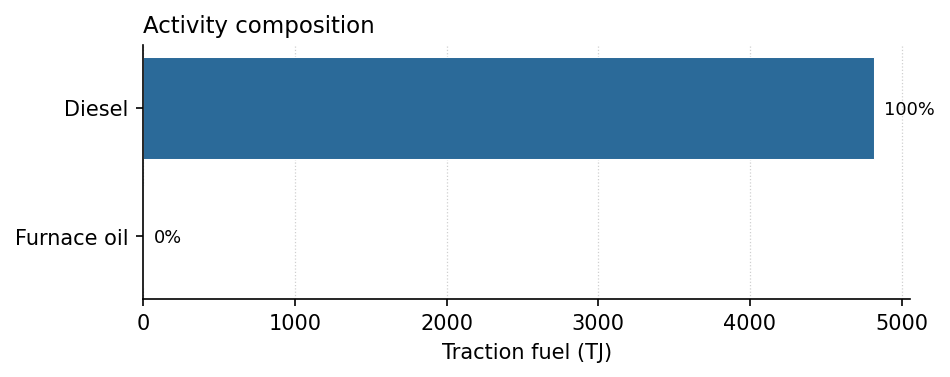
\includegraphics[width=\linewidth]{railways_activity.png}
\caption{The energy basis. One stream is the sector.}
\label{fig:activity}
\end{figure}

\subsection{Electric traction: none since about 2010, and none in scope}

Recent Year Book editions report Electric Energy as NIL, and the historical table behind that
figure says when it became true. Electric traction energy is non-zero from the 1985--90
quinquennium (\SI{37.4}{\giga\watt\hour} per year on average) and declines through 2005--2010
(\SI{6.1}{\giga\watt\hour}) before going NIL from the 2010--2015 row. The Lahore--Khanewal
electrification---the operator's only electrified section---therefore ran into the late
2000s, not the 1970s as this paper previously stated; the mainline network has been
diesel-only since roughly 2010, which covers every inventory year here. The sector
consequently has no scope-2 stream, unlike residential fuel where the electricity boundary has
to be argued.

The scope is the Pakistan Railways mainline system's direct combustion. Urban electric rail
outside the operator---the Lahore Orange Line metro---has zero direct 1A3c combustion
emissions by definition; its electricity-related emissions belong to power generation, and the
boundary is recorded in the completeness assessment rather than left implicit in a NIL row.

\subsection{Two things the source does badly, both recorded}

\textbf{Five editions are scans, and it turned out not to matter.} The 2017--18, 2018--19,
2019--20, 2021--22 and 2024--25 editions are page images with no extractable text layer, and
this paper previously reported FY2018 and FY2019 as absent from the time series for that
reason.

That was true about those editions and wrong about the data. Every edition's fuel table carries
a historical run, not just the current year, and the 2020--21 edition has a text layer: it
reports FY2015--16 through FY2020--21 annually. Both missing years were one edition later the
whole time. They are now in the series---\num{156396} and \num{159927} thousand
litres---recovered rather than interpolated, and the series runs FY2014--FY2025 unbroken.

What makes them trustworthy is that the same table reproduces FY2016, FY2017 and FY2021
exactly against figures this inventory already held from other editions. A test asserts that
correspondence, and a second asserts the series is contiguous, because the honest reason to
leave a hole in it has gone.

\textbf{Furnace oil changed unit labels without announcement, and the source itself settles
the basis.} Editions through 2020--21 label the row ``Tonnes'' and editions from 2022--23 label
it ``Liters/thousand,'' with no note explaining the change. The 2023--24 edition resolves it
against itself: its detailed fuel table and the narrative on the same page state the quantity
in metric tonnes, and the summary table's unit column is demonstrably unreliable
(Section~\ref{sec:limitations}). The basis is tonnes, and that is what the activity file
carries. The stream is under \SI{0.001}{\mega\tonne} \COe{} on either reading, so nothing
material turns on it, and a test pins that indifference by recomputing the total under both
interpretations. The unit travels with each row in the activity file rather than being
inferred from the year, so any future correction is a data edit and not a code change.

Furnace oil is carried at all for two reasons: IPCC Chapter~3 §3.4.1.4 warns specifically
against omitting non-diesel traction fuels, and an unexplained unit change in a government
series is worth recording where the next person will find it.

\subsection{The traffic statistics}

The same Year Book reports \num{26885} thousand passenger, mixed and other coaching
train-kilometres and \num{6237} thousand freight, \num{33122} thousand in total. These do not
enter the estimate. They are carried as a parameter because they permit the fuel figure to be
checked against the traffic that consumed it, which is the evidence behind
Section~\ref{sec:validation}.

\section{Methods}
\label{sec:methods}

\subsection{The calculation}

Litres to tonnes to energy to emissions, once per fuel and per gas:
\begin{equation}
E_{f,g} \;=\; Q_f \cdot \rho_f \cdot \mathrm{NCV}_f \cdot \mathrm{EF}_{g},
\label{eq:main}
\end{equation}
where $Q_f$ is the published quantity, $\rho_f$ the density needed to reach a mass basis,
$\mathrm{NCV}_f$ the net calorific value, and $\mathrm{EF}_{g}$ the IPCC rail factor for gas
$g$. There is nothing else in the sector.

The density matters more than it looks. Pakistan Railways reports litres and every IPCC factor
is per unit of energy, so a density is unavoidable, and it is taken from Pakistan State Oil's
own high-speed-diesel material safety data sheet---specific gravity \numrange{0.83}{0.86} at
\SI{16}{\celsius}, midpoint \SI{0.845}{\kilo\gram\per\litre}---rather than from a generic
international default. That spread is the entire uncertainty in the step, and at
\SI{2}{\percent} it is the smallest term in the sector.

\subsection{The furnace-oil rows}

Furnace oil takes its \COtwo{} factor from the fuel's own carbon content in Volume~2 Chapter~2
Table~2.2, because Table~3.4.1 tabulates only diesel and sub-bituminous coal. Its \CHfour{} and
\NtwoO{} factors are the diesel rail values, following §3.4.1.4, which directs that other
traction fuels burnt in the same engines be treated with the same emission properties. Both
choices are recorded on the factor rows rather than inferred from the code.

\subsection{Fossil methane}

Diesel and furnace oil are fossil fuels, so their \CHfour{} takes AR5's fossil value of
\num{30} rather than the biogenic \num{28}---the same treatment as road transport, power and
aviation, and the opposite of waste. A test asserts the \COe{} of every \CHfour{} row against
\num{30} exactly, because the two values differ by seven percent and nothing in the output
distinguishes them.

\subsection{The air-pollutant layer}
\label{sec:air}

Air pollutants take the EMEP/EEA Guidebook's railway chapter \citep{emep2023rail} at
Tier~1: factors per tonne of fuel, on the identical fuel-mass chain as the greenhouse
gases, in kilotonnes of native mass that never enter a \COe{} total. Black carbon is the
chapter's declared fraction (\num{0.65}) of PM\textsubscript{2.5}---a component of the
particulate mass, never an addition to it---and the chapter's one defect is recorded
rather than repaired: its printed 95\% intervals for the three particulate rows do not
bracket their own central values, so those rows carry the printed bounds verbatim and a
conservative $\pm$\SI{100}{\percent}.

\SOtwo{} is stoichiometry, not a factor: twice the fuel's sulfur mass. The chapter says
operator sulfur values are preferable to defaults; Pakistan Railways publishes none, and
Pakistani diesel spans three orders of magnitude---\SI{10}{ppm} Euro-V imports, mandatory
since January 2021, against the \SI{500}{ppm} pre-Euro-V specification and the older
specification's \SI{1}{\percent} ceiling that covers most of the historical series. So
\SOtwo{} ships as an explicit case ladder with the \SI{500}{ppm} specification as the
declared reference, not as one number pretending to precision the fuel supply does not
have.

A Tier~2 diagnostic accompanies the reported Tier~1 layer: fuel split among line-haul
passenger, line-haul freight and shunting (railcars are not occurring---workings are Nil
in every recent year), rescaled to the metered control exactly, as the chapter itself
instructs. Published train-kilometres divide the line-haul fuel; the shunting share is a
declared five-percent assumption, derived from the chapter's own duty rates and
gap-registered, because no shunting activity is published in any form. What the diagnostic
shows is the duty-cycle sensitivity: a nearly-all-line-haul fleet implies Tier~1
understates NO\textsubscript{x} by roughly a fifth and overstates fine particulate mass by
about a sixth, and neither layer is silently swapped for the other.

\subsection{The diesel closure against road transport}
\label{sec:closure}

Pakistan's national high-speed-diesel supply figure covers road, rail, agriculture and
captive generation together. While the road transport sector anchored on that single national
figure, every litre Pakistan Railways burns was at risk of being counted twice---once here and
once as road diesel---and the road sector deducted this module's diesel, litre for litre, by
calling it rather than by holding a copy of the number.

\textbf{That deduction has been retired, and this section records why rather than describing a
mechanism that no longer runs.} Road transport is now anchored on the petroleum industry's own
customer classes, in which Railways is a separate row from Road. The double-count is excluded
by construction at the source, so subtracting the railway account from the road control would
now remove the same fuel twice.

What the railway fuel account does instead is better. Freed from being an internal correction,
it is an \emph{independent cross-source check}: the operator's own metered purchases, from the
Year Book, against the petroleum industry's Railways customer-class total, two organisations
counting the same physical fuel by different routes. The quantity itself is unchanged---
the module's metered diesel is \SI{112.04}{\kilo\tonne}, traction and non-traction
together---and only what the inventory does with it has moved. An internal deduction can only be
arithmetically consistent; an independent comparison can be wrong, which is what makes it
worth reporting. Section~\ref{sec:validation} gives the comparison.

The general point outlives this instance. A closure that becomes structurally impossible has
been superseded by better source data rather than broken, and the right response is to delete
the correction and say so---not to keep a compensating adjustment running against a control
that no longer needs it.

One deduction from road transport's controls does survive, and it is not this sector's:
household generator petrol, owned by the residential module. A test asserts that the railway
account contributes nothing to it---Pakistan Railways burns no petrol, and deducting from a
fuel the operator does not use would be a second error correcting the first.

\subsection{Spatial support and the ODbL route alternative}
\label{sec:spatial}

The following route reconstruction is an ODbL-derived alternative, not the primary package's licensed grid. The primary product retains its compatible administrative support and records unsupported finer placement as unallocated. A source-specific physical rail release must not inherit an unrelated grid merely to eliminate that remainder.

Railway emissions can occur only along a railway, so the allocation is constrained to one.
Line-haul fuel runs along the OpenStreetMap-derived network---\num{7574} active
line-kilometres, \SI{97}{\percent} of the Year Book's \num{7791} route-kilometres---divided
into corridors; shunting fuel sits at the seven divisional yards, weighted by their
published wagon loadings; and each of the three service streams takes its fuel share from
the Tier~2 split, on a surface that reconciles to the national control exactly at national,
provincial and district level on every run.

The honest split of that construction: the network geometry, the yard locations and the
route-kilometre audit are data; the corridor service weights are \emph{declared judgment},
stated basis-by-basis on their data rows, because the operator's public timetable interface
refuses unauthenticated access and no service-frequency statistics are published. The
previous proxy---freight wagons loaded by division, which credited Sindh with fuel burnt
hauling Karachi-origin freight up-country and allocated passenger operations (four times the
freight train-kilometres) by freight geography---is retained as a structural alternative,
and both splits are published. The national total is identical under either; the engine
reads the transcribed share row, and a test pins that row against a fresh spatial
computation so the two cannot drift apart.

\section{Emission Factors}
\label{sec:factors}

\begin{table}[htbp]
\centering
\footnotesize
\begin{tabular}{@{}lrrr@{}}
\toprule
\textbf{Gas} & \textbf{Rail (3.4.1)} & \textbf{Road (3.2.1/3.2.2)} & \textbf{Ratio} \\
\midrule
\COtwo{}  & 74\,100 & 74\,100 & 1.00 \\
\CHfour{} &    4.15 &     3.9 & 1.06 \\
\NtwoO{}  &    28.6 &     3.9 & 7.33 \\
\bottomrule
\end{tabular}
\caption{IPCC 2006 defaults for diesel, kg per TJ, from Volume~2 Chapter~3
\citep{ipcc2006energy}. The \COtwo{} rows are identical because \COtwo{} depends only on the
carbon in the fuel; the \NtwoO{} rows are not.}
\label{tab:factors}
\end{table}

\subsection{Why rail \NtwoO{} is \num{7.3} times road}

Large slow-speed locomotive engines run lean at high load, which is the \NtwoO{}-forming
regime. IPCC derives the rail values in Table~3.4.1 from EEA measurements at
\SI{0.35}{\litre} per brake-horsepower-hour for a \SI{4000}{HP} locomotive, and the
\SI{28.6}{\kilo\gram\per\tera\joule} value carries a 95\% interval of
\SIrange{14.3}{85.8}{\kilo\gram\per\tera\joule}. The road value of
\SI{3.9}{\kilo\gram\per\tera\joule} describes a different engine population running a different
duty cycle.

\subsection{What the wrong table would do}

Substituting the road \NtwoO{} factor would understate railway \NtwoO{} by \SI{86}{\percent}
and the sector total by about \SI{8}{\percent}, from \SI{0.394}{} to
\SI{0.363}{\mega\tonne}. That figure is not left as a claim in a docstring: the runner computes
it and publishes it as a diagnostic row in the sector's totals file, so a reader can see the
size of the choice rather than take it on trust.

\subsection{The trap, caught in the current filing}

This is no longer only a hypothesis about how the BUR went wrong. Pakistan's current
Common Reporting Tables carry, in the implied-emission-factor cells of the railway
category's own liquid-fuels row, \COtwo{} at \num{74.10} t/TJ, \CHfour{} at \num{3.90} and
\NtwoO{} at \num{3.90} kg/TJ---the road table's non-\COtwo{} pair, on rail, in the
official submission of record. The cell-audited extraction behind that statement
reproduces the filing's arithmetic from its own workbook before comparing anything to it,
and a test pins the finding so that a corrected future submission fails the pin and forces
this paragraph to be rewritten rather than left standing.

\subsection{Why this is a trap and not a mistake}

The failure is silent in every direction a compiler would normally look. Both tables are in the
same chapter of the same volume. Both are labelled for transport. The \COtwo{} row---which is
\SI{90}{\percent} of the category---is byte-identical, so a total computed with the wrong table
still reconciles against fuel, still matches a carbon-balance check, and still passes any
comparison run on \COtwo{} alone. Only the \NtwoO{} row moves, and only by an amount that looks
like ordinary uncertainty in a category this small.

Four tests hold the choice in place. One asserts that the cited source contains ``Rail.'' One
asserts that rail \NtwoO{} exceeds five times the road value, so a silent substitution of the
transport rows fails immediately. One asserts that rail \CHfour{} exceeds road \CHfour{}. And
one asserts that \NtwoO{} is more than \SI{5}{\percent} of the sector total---because a pinned
factor that nothing depends on is decoration, and the guard is only worth having while the
choice still moves the answer.

\FloatBarrier
\section{Validation}
\label{sec:validation}

\subsection{A national submission, refuted twice}

Pakistan's First Biennial Update Report reports railways at \SI{4.06}{\mega\tonne} \COe{} for
FY2017--18. That fiscal year is inside this inventory's series, so the primary comparison is
matched-year: the identical method, GWP basis and scope, applied to the \num{156396} thousand
litres the operator reports for FY2017--18, gives \SI{0.466}{\mega\tonne}---a factor of
\num{8.7} below the submission in its own inventory year. The reference-year result is
reported separately: \SI{0.394}{\mega\tonne} module total for FY2023--24
(\SI{0.389}{\mega\tonne} strict 1A3c). A year effect is ruled out by
the fuel itself: FY2017--18 diesel is \SI{18.0}{\percent} above FY2023--24, not a factor of ten
in either direction.

\textbf{The carbon route.} \SI{4.06}{\mega\tonne} of \COtwo{} requires the combustion of
roughly \SI{1280}{\kilo\tonne} of diesel. Pakistan Railways reports consuming
\SI{132}{\kilo\tonne} in FY2017--18, and \SI{112}{\kilo\tonne} in the reference year. The
submitted figure needs nearly ten times the fuel the operator's own accounts record for the
same year, and no accounting treatment of a fuel account produces carbon that was not in the
fuel. A test bounds the sector total between \SI{0.2}{} and \SI{1.0}{\mega\tonne} for this
reason, so a future revision that drifted toward the submitted value would fail rather than
pass quietly.

\textbf{The traffic route.} The second check is independent of the fuel account, because it
uses a different table in the same publication. Pakistan Railways ran \num{33.1} million
train-kilometres in FY2023--24. The metered consumption works out at
\SI{4.0}{\litre} per train-kilometre, which is where a diesel locomotive hauling mixed
passenger and freight traffic belongs. The fuel implied by the submitted figure, spread over
the same traffic, would be \SI{46}{\litre} per train-kilometre---an order of magnitude above
what any locomotive consumes. A test pins the intensity between \num{2} and \num{10} litres
per train-kilometre.

Two routes, two published tables, one conclusion. The metered consumption, the traffic
statistics and the carbon content of diesel all support the lower figure, so it is the one
reported here.

\subsection{Why this is recorded rather than reconciled}

The alternative to publishing this disagreement is to adopt the submitted value, or to split
the difference, or to say nothing. All three would be worse.

Adopting it would require inventing ten times the fuel Pakistan Railways reports consuming in
the submission's own year.
Splitting the difference would produce a number supported by no source at all. Saying nothing
would leave a reader who compares this inventory with Pakistan's UNFCCC submission to discover
a factor of ten unexplained, and to have no way of telling which figure to trust.

What is defensible is to state the disagreement, show the arithmetic on both routes, put the
checks in the test suite so they run on every build, and let the reader see the evidence. This
is the same standard applied in this inventory's fugitives sector to a disagreement with EDGAR
that could \emph{not} be resolved---and the contrast is the point. There, two models chose
differently within one published range and the comparison settled nothing. Here, one figure is
outside what the fuel can produce.

\subsection{Every official statement of this category, matched by year}

\begin{table}[htbp]
\centering
\footnotesize
\begin{tabular}{@{}llrrr@{}}
\toprule
\textbf{Source} & \textbf{Year} & \textbf{Official} & \textbf{This work} & \textbf{Ratio} \\
\midrule
INC (derived)  & FY1993--94 & 0.557 & 0.633 & 0.88 \\
BUR-1          & FY2017--18 & 4.060 & 0.466 & 8.7  \\
TNC            & CY2021 & \multicolumn{3}{l}{\emph{railways not separately reported}} \\
BTR-1 (narrative) & CY2021 & \multicolumn{3}{l}{\emph{railways not separately reported}} \\
CRT (= BTR-1 annex) & CY2022 & 4.259 & 0.368 & 11.6 \\
\bottomrule
\end{tabular}
\caption{Every official statement of this category, Mt \COe{}, each compared in its own
inventory year by the identical method. The INC row is derived from its stated share
(3\% of \num{18584.4} Gg) and compared against the quinquennial history layer's
1990--95 indicative value---a magnitude check, not a point match. The TNC and the BTR-1
narrative report 1.A.3 as one aggregate line; the BTR-1's railway statement exists only
in its CTF annex, which is the CRT row. The CRT total is stated on the filing's own GWP
basis, its calendar year straddling two fiscal years (own value: their mean).}
\label{tab:official}
\end{table}

The table's arc is the paper's history of the category in five rows. The INC-era
inventory was \emph{sane}: its derived railway figure sits within \SI{11.9}{\percent} of this
inventory's independent reconstruction from the Year Book's own fuel history,
furnace-oil traction included. The order-of-magnitude error entered the record with
BUR-1, persists in the current CRT, and the two documents in between decline to state a
railway figure at all---which is the procedural gap made visible: a submission that
published subsector activity alongside its estimate would be auditable, and the one time
it was (the CRT), the audit takes one worksheet.

The CRT comparison adds what the BUR comparison could not: mechanism. The filing's
implied-factor cells show the road table on rail (Section~\ref{sec:factors}), and its
activity---\num{56609} TJ, about \num{1316} kt of diesel---implies eleven to thirteen
times the fuel the operator metered in the overlapping years. The order-of-magnitude
error and the factor-table error are distinct, visible separately in the filing's own
arithmetic, and both are pinned by tests against the extracted cells.

\subsection{An independent global inventory, and what it misses}

ELK, the one open global inventory with separate passenger- and freight-rail layers,
carries a non-zero Pakistan rail signal: \SI{172}{\kilo\tonne} of \COtwo{} for 2019,
country-masked, against this inventory's \SI{404}{\kilo\tonne} for the same calendar
year---\num{0.43} times, a factor-of-two disagreement rather than the officials' factor of
ten, and evidence that the global model did not ingest the BUR. Its composition, however,
is inverted: \SI{165}{\kilo\tonne} on freight across a thousand grid cells against
\SI{7}{\kilo\tonne} of passenger rail on five cells, for an operator whose traffic is
four-to-one \emph{passenger} by train-kilometre. A fleet model without national activity
data reconstructs the wrong railway; the operator's two published numbers---fuel and
train-km---are what it lacks. The comparison is a benchmark, never a calibration target,
and the extraction states its hypotheses before computing.

\subsection{The auditor's litre-level corroboration}

The one-operator limitation is real: the Year Book supplies both the fuel account and the
traffic that checks it. The Auditor-General's railway audits are the independent
institution, and their findings corroborate the meters precisely by documenting control
failures: \num{710143} litres consumed against a \num{316664}-litre quota across six
formations in FY2023--24; \num{393554} litres above per-class trip rations in an earlier
year; \num{23250} litres pilfered from stabled locomotives and detected against the tank
record. Quota breaches resolved at the litre level per formation are only possible where
fuel issue is metered. The audited excesses are fractions of a percent of the national
figure: fuel \emph{control} is weak, fuel \emph{measurement} is not, and it is the
measurement this inventory rests on.

\subsection{Intensity, over time and against the world}

The EMEP chapter's verification guidance is fuel against distance and traffic. Pakistani
rail runs at \numrange{4.0}{5.1} litres per train-kilometre across FY2022--FY2025, with
FY2023--24 at \num{4.0}; freight moves at roughly \SI{8}{\gram} \COtwo{} per
tonne-kilometre and passengers at under \SI{10}{\gram} per passenger-kilometre---the
heavy-load end of world rail, consistent with long, full trains. The World Bank's
UIC-sourced series, institutionally independent of the Year Book, corroborates the
passenger-kilometre magnitude. Every quotient is diagnostic; none feeds the inventory.

\subsection{Internal checks}

Three further properties are asserted on every run. Diesel exceeds \SI{99}{\percent} of
traction energy, so a corruption of the furnace-oil row cannot move the sector. The sector
total is indifferent to the furnace-oil unit ambiguity, recomputed both ways and agreeing to
better than \SI{0.001}{\mega\tonne}. And the provincial allocation reconciles exactly against
the national figure.

The road-transport comparison of Section~\ref{sec:closure} is enforced by test on every run:
the two rail figures---the Year Book's metered \SI{112.04}{\kilo\tonne} and the OCAC Railways
customer-class row at \SI{107.93}{\kilo\tonne}, two unrelated reporting chains
\SI{3.8}{\percent} apart---must agree within \SI{5}{\percent} and must \emph{not} be equal,
because equality would mean one had been copied from the other; the matched-year pair must
beat the two-year bracket; the road diesel control must equal the OCAC Road row exactly, with
no rail subtraction anywhere; petrol carries no rail contribution; and rail's share of
national high-speed diesel stays between \num{0.2} and \SI{5}{\percent}---because if that
ratio ever left the range, one of the two national figures for the same fuel would have
broken.

\section{Results}
\label{sec:results}

\subsection{The sector}

Pakistan's railways emitted \SI{0.39437}{\mega\tonne} \COe{} in FY2023--24 on AR5
metrics, or \SI{0.39547}{\mega\tonne} on AR6---and the
reference itself books the measured split the Year Book's detail table provides:
\SI{0.38939}{\mega\tonne} of locomotive traction at 1.A.3.c, and
\SI{0.00498}{\mega\tonne} of workshop, power-house, pump and track-machinery fuel at
its own category (1A2/1A4c, the split below the one published aggregate unresolved),
rather than declaring the latter IE inside the traction code.

\begin{table}[htbp]
\centering
\footnotesize
\begin{tabular}{@{}llrrr@{}}
\toprule
\textbf{Stream} & \textbf{Gas} & \textbf{Gg} & \textbf{Mt \COe{}} & \textbf{$\pm$\%} \\
\midrule
Diesel (traction) & \COtwo{}  & 352.678 & 0.35268 &   5.4 \\
            & \NtwoO{}  &   0.136 & 0.03607 & 150.1 \\
            & \CHfour{} &   0.020 & 0.00059 & 130.1 \\
Furnace oil (traction) & \COtwo{} & 0.047 & 0.00005 &  30.1 \\
Non-traction, all fuels & all & & 0.00498 & \\
\midrule
1A3c locomotive traction & & & 0.38939 & \\
Non-traction (1A2/1A4c) & & & 0.00498 & \\
\textbf{Module total} & & & \textbf{0.39437} & \\
\bottomrule
\end{tabular}
\caption{Railway module streams, FY2023--24. Two furnace-oil rows below \SI{0.0001}{\mega\tonne} are
omitted from the table and included in the total. The non-traction row's allocation between
1A2 and 1A4c is unresolved; it books at its own category pending a per-use split.}
\label{tab:streams}
\end{table}

\begin{figure}[htbp]
\centering
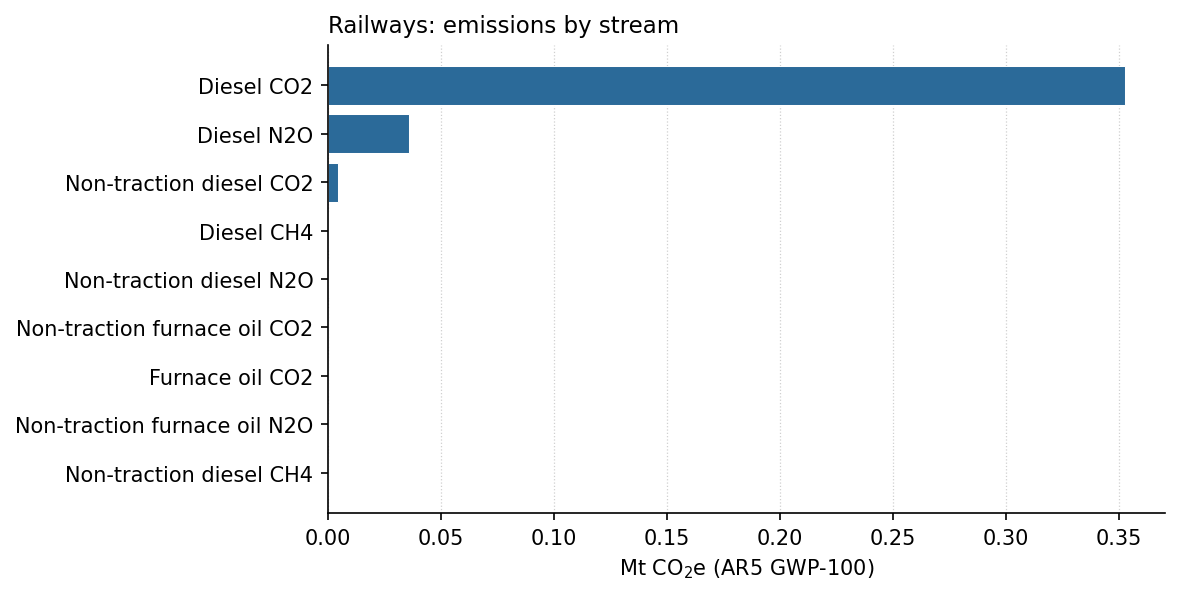
\includegraphics[width=\linewidth]{railways_streams.png}
\caption{Emissions by stream. \COtwo{} is \SI{90.6}{\percent} of the category and \NtwoO{} is
\SI{9.3}{\percent}, which is the entire reason the factor-table choice matters.}
\label{fig:streams}
\end{figure}

The uncertainty structure is unusual for this inventory. Diesel \COtwo{} at
$\pm\SI{5.4}{\percent}$ is the best-constrained stream in the whole national estimate---a
single state operator's metered consumption against a factor whose 95\% interval spans
\SI{3}{\percent}---while \NtwoO{} at $\pm\SI{150.1}{\percent}$ is among the worst. The sector
is simultaneously the most accurately measured and, in its second gas, the least confidently
factored.

\subsection{The factor-table diagnostic}

\begin{table}[htbp]
\centering
\footnotesize
\begin{tabular}{@{}lr@{}}
\toprule
\textbf{Case} & \textbf{Mt \COe{}} \\
\midrule
Rail table (3.4.1), reported     & 0.39437 \\
Road table (3.2.2) substituted   & 0.36282 \\
\bottomrule
\end{tabular}
\caption{What the sector would report on the road \NtwoO{} factor. The gap is
\SI{8.0}{\percent} of the category and \SI{100}{\percent} of the reason the table choice is
pinned by a test.}
\label{tab:diagnostic}
\end{table}

\subsection{The air-pollutant layer}

\begin{table}[htbp]
\centering
\footnotesize
\begin{tabular}{@{}lrr@{}}
\toprule
\textbf{Pollutant} & \textbf{kt, FY2023--24} & \textbf{$\pm$\%} \\
\midrule
NO\textsubscript{x} & 5.8749 & 65.2 \\
CO                  & 1.1996 & 61.2 \\
NMVOC               & 0.5213 & 65.2 \\
TSP                 & 0.1704 & 100.1 \\
PM\textsubscript{10}  & 0.1614 & 100.1 \\
PM\textsubscript{2.5} & 0.1536 & 100.1 \\
BC                  & 0.0998 & 104.4 \\
\SOtwo{}            & 0.1176 & 100.1 \\
NH\textsubscript{3} & 0.0008 & 57.2 \\
\bottomrule
\end{tabular}
\caption{Railway air pollutants, EMEP/EEA Tier~1 on the metered fuel; native mass, never
\COe{}. BC is a component of PM\textsubscript{2.5}; \SOtwo{} is the \SI{500}{ppm}
reference case of a \SIrange{0.008}{2.25}{\kilo\tonne} sulfur ladder.}
\label{tab:air}
\end{table}

\begin{figure}[htbp]
\centering
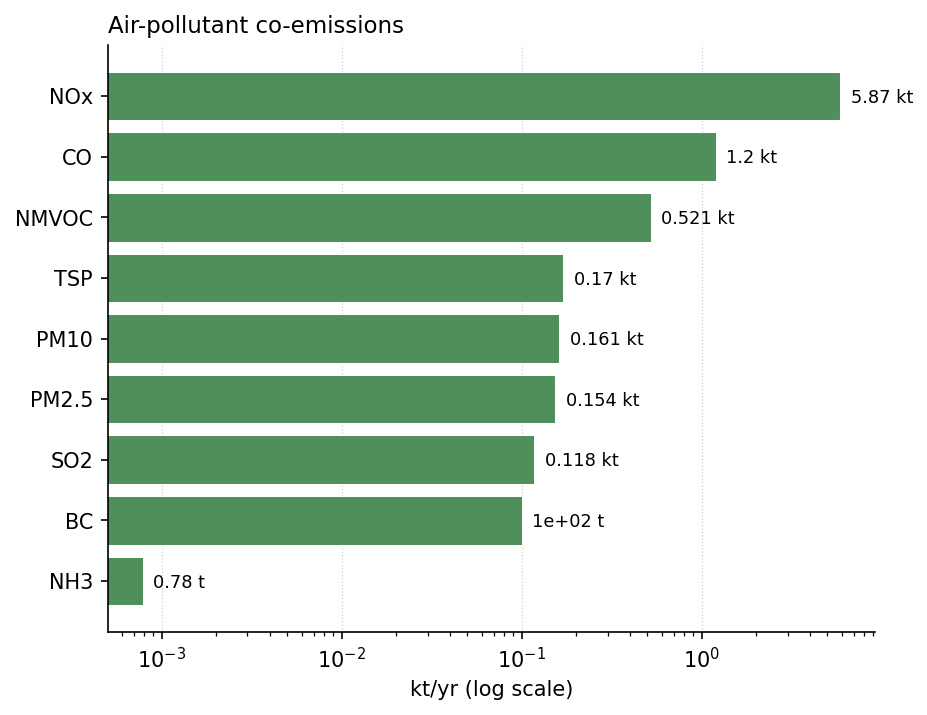
\includegraphics[width=\linewidth]{railways_air.png}
\caption{The air layer on a log axis: NO\textsubscript{x} in the kilotonnes, the
particulate family in the low hundreds of tonnes, black carbon just under \num{100}
tonnes.}
\label{fig:air}
\end{figure}

For scale: railway NO\textsubscript{x} at \SI{5.9}{\kilo\tonne} is a small national term,
but it is emitted in a hundred-metre-wide corridor through the centres of Pakistan's
largest cities, which is what the route-constrained surfaces of
Section~\ref{sec:spatial} exist to place. \SOtwo{} is the one pollutant whose national
value is genuinely open: on Euro-V fuel throughout it would be \SI{0.008}{\kilo\tonne}, on
the historical \SI{1}{\percent} specification \SI{2.25}{\kilo\tonne}---a \num{287}-fold
span that only an operator fuel-quality certificate can close.

\subsection{The series, and what it shows about Pakistani rail}

\begin{figure}[htbp]
\centering
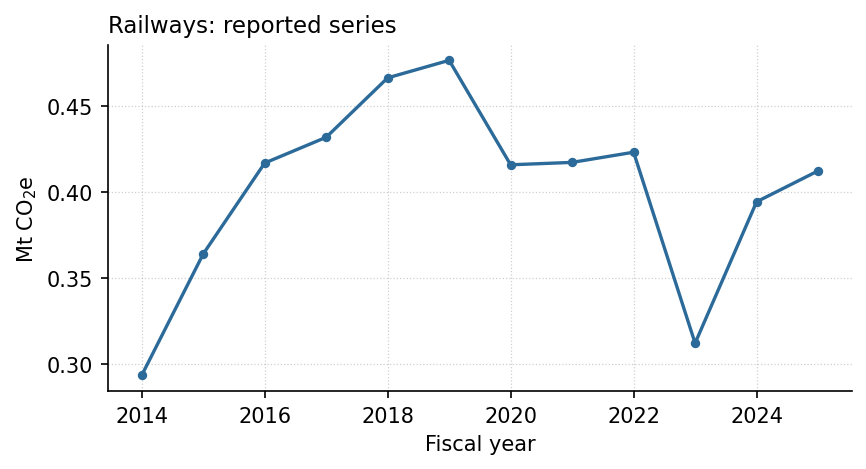
\includegraphics[width=\linewidth]{railways_timeseries.png}
\caption{FY2014--FY2025, unbroken. Emissions rise from \SI{0.294}{} to
\SI{0.412}{\mega\tonne} as diesel consumption rises from \num{98212} to \num{138673} thousand
litres, peaking at \SI{0.477}{\mega\tonne} in FY2019; the reference year FY2023--24 stands at
\SI{0.394}{\mega\tonne}. FY2018 and FY2019 were previously absent, recovered from the
2020--21 edition's historical table; FY2025 is provisional by its edition's own declaration.}
\label{fig:series}
\end{figure}

Three features, one of them only visible now the gaps are filled. The trend is upward---two
fifths more fuel across the twelve-year series, against a national inventory in which most
transport categories also grew. The series is volatile, dropping from \SI{0.423}{} in FY2022 to
\SI{0.312}{\mega\tonne} in FY2023 before recovering. And it peaks in FY2019 at
\SI{0.477}{\mega\tonne}, \SI{22}{\percent} above the reference year---a maximum that sat
inside the two recovered years and was therefore invisible in every previous version of this
figure. A single operator's annual fuel account is still a lumpy quantity, sensitive to
service suspensions, locomotive availability and the timing of procurement and depot issues,
and under the annual-equivalence assumption of Section~\ref{sec:data} the series should be
read as the operator's fuel account rather than as a smooth measure of traffic.

\subsection{Provincial allocation}

\begin{figure}[htbp]
\centering
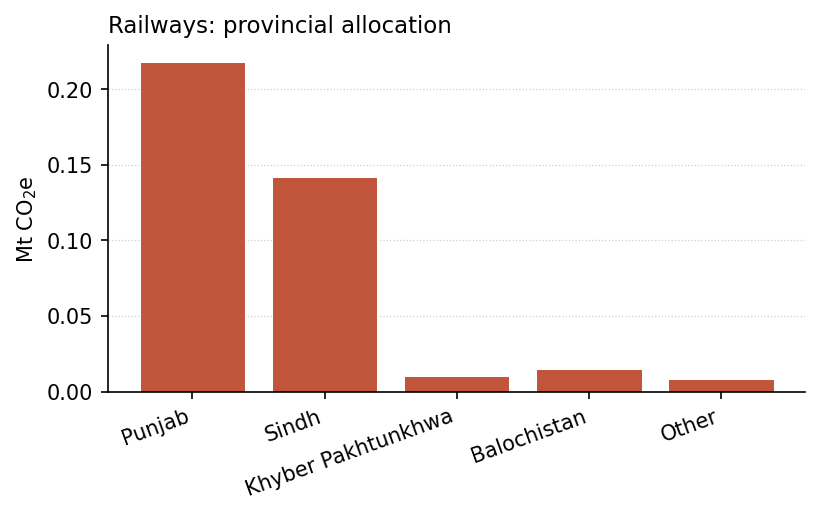
\includegraphics[width=\linewidth]{railways_provincial.png}
\caption{Punjab \SI{0.218}{\mega\tonne}, Sindh \SI{0.142}{\mega\tonne}, Balochistan
\SI{0.015}{\mega\tonne}, Khyber Pakhtunkhwa
\SI{0.010}{\mega\tonne}. Allocated on the route-constrained model of
Section~\ref{sec:spatial}; the residual share is the Islamabad Capital Territory trackage.}
\label{fig:provincial}
\end{figure}

The route model reverses the previous picture. The freight-wagons proxy put Sindh at
\SI{66}{\percent} because Karachi loads most wagons; constrained to the network that
actually burns the fuel, \SI{56}{\percent} of emissions land in Punjab, whose trunk
corridors carry the long-haul services both ways. The corridor weights beneath that split
are declared judgment pending the operator's timetable, so the wagons alternative is
retained as a structural scenario---Sindh \SI{66}{\percent} against \SI{36}{\percent}---and
the difference between the two is the honest statement of the split's uncertainty. What the
route model adds that no provincial proxy could: emissions sit on cells with track or
yards, nowhere else, which is the property an air-quality model actually needs.

\subsection{Place in the national inventory}

At \SI{0.09}{\percent} of the national total, railways is not a key category by level and
contributes nothing measurable to national variance. It is included because completeness is a
property of an inventory rather than of its largest categories, and because the attribution
it settles---national diesel the road category once absorbed wholesale, now excluded from the
road control at its source and verified by an independent two-source comparison---is roughly
a third of a megatonne, the size of this entire sector.

\section{Uncertainty}
\label{sec:uncertainty}

\subsection{What a percentage can say}

One metered account drives every stream, so the activity components of the row
uncertainties are correlated; the grouped Approach~1 treats each fuel's activity term as
perfectly shared across its gas rows and lands at $\pm$\SI{14.7}{\percent} on the sector
total, against \SI{14.55}{\percent} if the rows were independent. The interval's shape is
the sector's story in miniature: diesel \COtwo{} at $\pm$\SI{5.4}{\percent} is among the
best-constrained streams in the national inventory, while diesel \NtwoO{} carries
$\pm$\SI{150}{\percent} and is a tenth of the category---the sector is simultaneously the
most accurately measured and, in its second gas, the least confidently factored. The full
inputs register, with every quantity the statement rests on, ships as a generated output.

\subsection{What a percentage cannot say}

Discrete choices are named cases with conditional intervals and no probabilities attached,
in this inventory's standard idiom:

\begin{table}[htbp]
\centering
\footnotesize
\begin{tabular}{@{}lrp{0.42\linewidth}@{}}
\toprule
\textbf{Scenario} & \textbf{Mt \COe{}} & \textbf{What it answers} \\
\midrule
reference                     & 0.39437 & the estimate \\
road\_n2o\_factor             & 0.36282 & the road table on rail---the CRT's own treatment \\
ie\_summary                   & 0.39437 & the earlier summary booking restated: everything
                                          inside 1.A.3.c, the 0.00498 non-traction
                                          share declared IE; the reference itself now
                                          books the recode \\
stock\_timing\_prior\_year    & 0.35323 & consumed-equals-burnt bounded by the prior-year mean \\
tier2\_service\_split         & 0.39437 & invariant by construction; the split moves nothing \\
\bottomrule
\end{tabular}
\caption{Structural scenarios for the greenhouse-gas total. The \SOtwo{} sulfur ladder
(\SIrange{0.008}{2.25}{\kilo\tonne}) and the provincial wagons-proxy alternative are
scope-noted separately in the generated scenario table; the once-live summary-vs-detail
scenario is retired, its question settled by the 2024--25 edition's restatement.}
\label{tab:scenarios}
\end{table}

The largest genuine uncertainty in the sector is not in its total at all. It is the
\NtwoO{} factor's published range, which nothing short of measurement on Pakistani
locomotives would narrow---and at \SI{0.09}{\percent} of national emissions the case for
that campaign is air quality and fleet performance, not greenhouse-gas accounting.

\FloatBarrier
\section{Discussion}
\label{sec:discussion}

\subsection{When a submission can be refuted, and when it cannot}

Independent checking of national greenhouse-gas submissions usually ends inconclusively. Two
estimates differ; both are models; neither is a measurement; and the comparison records a
disagreement without resolving it. This inventory's fugitives sector is a clean example, where
a factor of \num{1.3} against EDGAR settles nothing because both estimates choose within the
same published IPCC range and neither has observed a Pakistani gas system.

Railways is the opposite case, and the difference is worth stating precisely because it is not
about rigour. It is about what the category rests on.

A fugitive emission factor is a statement about infrastructure nobody has measured. A railway
fuel figure is a quantity a state enterprise metered, paid for and published, and the carbon
in it is fixed by chemistry. When a submitted figure requires ten times that fuel, the
disagreement is not between two models---it is between a figure and an audited quantity. And
when a second, independent statistic in the same publication puts the implied fuel intensity at
\SI{46}{\litre} per train-kilometre, the refutation no longer depends on trusting the fuel
account either.

The general form: a category can be refuted from outside when its activity datum is a metered
physical quantity and a second published statistic bounds the same quantity independently.
Railways has both. Most categories have neither, which is why this kind of result is rare
rather than because verification is usually done badly.

\subsection{What probably went wrong in the submission}

This paper does not know how the BUR's \SI{4.06}{\mega\tonne} was produced, and
speculating about it is not the same as refuting it, so that refutation stands on the
arithmetic alone. But the current CRT localises its own version of the error, because a
CRT publishes intermediates the BUR did not: the activity cell is \num{12.6} times the
metered fuel---a magnitude characteristic of a unit error, litres read as something
larger---and the implied-factor cells show the road table where the rail table belongs.
Two errors, separable in the filing's own arithmetic, each of which the operator's two
published statistics would have exposed immediately.

The constructive point is procedural rather than diagnostic. Had the submission published its
activity datum alongside its emissions, the disagreement would have been visible immediately
and resolvable by anyone. It is the absence of the intermediate quantity, not the estimate,
that makes the figure hard to check---and publishing implied fuel per train-kilometre alongside
the emissions would cost nothing and make the category self-auditing.

\subsection{What global inventories are missing, demonstrated}

The ELK comparison is worth generalising. A careful global fleet model, given no Pakistani
activity data, lands a factor of two low nationally and inverts the passenger--freight
composition entirely---five grid cells of passenger rail for an operator that runs four
passenger train-kilometres for every freight one. The two numbers that would have fixed it,
annual fuel and train-kilometres, have been published in the operator's Year Book every
year since the 1950s. The marginal value of nationally reported operator data to global
inventories is usually asserted; here it is measurable, in both magnitude and composition.

\subsection{The third instance of the parallel-table trap}

Volume~2 Chapter~3 contains several near-duplicate default tables. Their \COtwo{} rows agree,
because \COtwo{} depends only on the carbon in the fuel; their \CHfour{} and \NtwoO{} rows do
not, because those depend on the engine and the duty cycle.

This inventory has now hit that structure three times: residential fuel against the power
table, power against several, and rail against road here. In every case the failure would be
silent---the dominant gas is unaffected, the fuel reconciliation still closes, and the error
appears only in a minor gas at a magnitude that looks like ordinary uncertainty.

The defence that generalises is not vigilance. It is to publish the counterfactual. This sector
computes what it would report on the wrong table, \SI{0.363}{\mega\tonne} against
\SI{0.394}{}, and writes it into its own output as a labelled diagnostic row. A reader can then
see the size of the choice without re-deriving it, and a future edit that silently switched
tables would move a number that is checked rather than one that is not.

\subsection{Small categories and the attributions they settle}

At \SI{0.09}{\percent} of national emissions, railways would fail any threshold test for
inclusion. Its value to the inventory is not its own magnitude but the attribution it
settles: the national high-speed-diesel figure covers road and rail together, and before the
road sector re-anchored on the petroleum industry's customer classes, the road category
absorbed the whole of it. The two fuels are now separate rows at the source, and this
sector's metered account is the independent check that the Railways row is right.

That is a general property of small transport categories. They are frequently the reason a
large category's activity data can be stated correctly, and dropping them on grounds of size
leaves the large category quietly wrong by the amount that was dropped. Rail was worth about
a third of a megatonne to road transport, which is roughly the entire railway sector---the
correction to the neighbour was the same size as the category making it, and it now lives in
the source data rather than running as a deduction.

\section{Limitations}
\label{sec:limitations}

\textbf{The spatial model's geometry is measured; its corridor weights are not.} The
network, the yards and the route-kilometre audit are data. The service intensity assigned
to each corridor is declared judgment, because Pakistan Railways publishes no
service-frequency statistics and its public timetable interface refuses unauthenticated
access; the basis of every weight is stated on its data row, the freight-wagons proxy is
retained as the structural alternative, and the split's real uncertainty is the distance
between the two published alternatives. A timetable extraction, or divisional train-km if
any edition ever carries them, would replace the judgment with measurement. The national
total is unaffected throughout.

\textbf{Workshop and stationary fuel is inside the module's metered total, measured, and
booked at its own category.} Fuel burnt by railway workshops, power houses, pumps and track
machines is part of the same consumption total this sector reads---the source says so
itself: ``these quantities comprise the entire fuel consumed on the Railways, i.e.\ on
locomotives, power houses, water pumps, workshops etc.''---and IPCC §3.4.1.4 flags the
overlap explicitly. That fuel belongs outside 1A3c, but not in any single category. This
paper previously assigned the whole quantity to 1A4c~ii, which was a classification by
purchaser rather than by source: under the IPCC definitions, track-maintenance machinery is
off-road transport, workshop generators and power houses are stationary combustion, and
pumps follow their end use. What remains unresolved is only that FINAL split: the measured
non-traction quantity books at its own category (1A2/1A4c unresolved) rather than inside
1A3c, and no published record yet decomposes it across those end uses.

This paper previously also called that fuel inseparable. It is not. The same edition carries a
detailed fuel table on p.163 splitting locomotive from other-than-locomotive consumption, for
diesel and furnace oil, back to 1950---annually from 2015--16, in five-year averages before
that---one page from the summary this sector was built on. Non-traction diesel is
\SI{1599}{} thousand litres, \SI{1.21}{\percent} of the total (since the 2024--25
restatement below, the two tables' denominators agree). The
overlap is small, which is what the sector had assumed; the difference is that it is now
measured---and published as a ledger:
\texttt{outputs/railways\_fuel\_claimants\_2024.csv} carries each claimant with its
volume, share and emissions at the sector's own factors, closing to the headline exactly.
The recode IS the reference: the engine books
\SI{0.00498}{\mega\tonne} at its own non-traction category and 1.A.3.c at locomotive
traction, with the older summary booking preserved as the configuration
\emph{rail\_ie\_summary} in
\texttt{outputs/national\_configurations.csv}. Either booking conserves the national
total at \num{444.95542} exactly---the same fuel at the same
factors under a different code, never a deletion. (An earlier edition priced this axis
as a subtraction; the conserving recode replaced it, and the reference itself now
carries the split.)

\textbf{The Year Book disagreed with itself about the reference year, and its next edition
settled it.} Checking the summary against the detail across every year both tables cover
produced exactly one failure: the 2023--24 edition printed the FY2023--24 locomotive cell as
``136.988''---a decimal point where every other row in its column uses a comma---making the
detail sum \num{138587} against the summary's twice-stated \num{132588}, a
\SI{4.52}{\percent} gap. This paper reported the summary, on the strength of two statements
against one typographically anomalous row, and published the detail reading as a labelled
sensitivity of \SI{0.412}{\mega\tonne} against \SI{0.394}{}.

The 2024--25 edition resolved it. Its historical run restates the cell as
\num{130988}---printed with the same decimal-point quirk on the same row---and
$\num{130988}+\num{1599}=\num{132587}$, within one part in \num{132588} of the summary. The
misprint hypothesis was right, the reported number never moved, and the sensitivity is
retired. The reconciliation now closes in every year:

\begin{table}[htbp]
\centering
\footnotesize
\begin{tabular}{@{}lrrrr@{}}
\toprule
\textbf{FY} & \textbf{Summary} & \textbf{Loco} & \textbf{Other} & \textbf{Detail} \\
\midrule
2015--16 & 139\,487 & 137\,908 & 1\,579 & 139\,487 \\
2016--17 & 144\,631 & 142\,607 & 2\,024 & 144\,631 \\
2017--18 & 156\,396 & 154\,357 & 2\,039 & 156\,396 \\
2018--19 & 159\,927 & 157\,979 & 1\,948 & 159\,927 \\
2019--20 & 139\,600 & 137\,969 & 1\,630 & 139\,599 \\
2020--21 & 140\,257 & 138\,841 & 1\,416 & 140\,257 \\
2021--22 & 142\,086 & 140\,482 & 1\,601 & 142\,083 \\
2022--23 & 104\,909 & 103\,272 & 1\,637 & 104\,909 \\
2023--24 & 132\,588 & 130\,988 & 1\,599 & 132\,587 \\
2024--25 & 138\,673 & 137\,096 & 1\,577 & 138\,673 \\
\bottomrule
\end{tabular}
\caption{Thousand litres of diesel, across every year the two tables both cover. Eight
reconcile to the digit and two to within three parts in \num{140000}; the FY2023--24 row
carries the 2024--25 edition's restatement of the cell its predecessor misprinted as
``136.988.''}
\label{tab:yearbook}
\end{table}

The check that found this ran late, and the honest reflection stands: this paper's argument
is that a national submission can be refuted on a fuel account, and an inventory making that
argument has to hold its own fuel account to the same standard. It now does, on every
build---and the one anomaly the check ever surfaced was a misprint in a national statistical
publication, identified here from the document's own internal evidence before the publisher
restated it.

\textbf{The furnace-oil basis is settled, and it was not what the summary said.} Editions
changed the published unit label without announcement, and this paper recorded the ambiguity as
unresolved. The 2023--24 edition resolves it against itself: the p.163 column is headed
``Furnace Oil (M.~Tonnes)'', the narrative on the same page states \SI{79.907}{} M.T, and that
is exactly the detail table's \num{15.083} locomotive plus \num{64.824} other. The Principal
Statistics table calls the same quantity ``Liters/thousand''---and its unit column is
demonstrably unreliable, labelling Persons Employed ``Tonne'' and Cost of Employees ``No.'' The
basis is tonnes. The stream is under \SI{0.001}{\mega\tonne} either way, as this paper already
argued, so nothing material moves; the data now say the right thing.

\textbf{\NtwoO{} is a tenth of the sector and carries $\pm\SI{150}{\percent}$.} The rail
default's 95\% interval spans \SIrange{14.3}{85.8}{\kilo\gram\per\tera\joule}, which is the
whole of the sector's uncertainty in practice. Nothing short of measurement on Pakistani
locomotives would narrow it, and the sector is too small for that to be worth doing.

\textbf{The air-pollutant layer rests on European fleet-average factors and a declared
sulfur assumption.} The EMEP/EEA Tier~1 locomotive factors describe an average European
fleet, not Pakistan's; the chapter's own confidence intervals are carried on every factor
row, and its printed intervals for the particulate rows do not bracket their central
values---a defect of the source recorded on the rows rather than silently repaired. \SOtwo{}
depends entirely on fuel sulfur, for which no operator certificate is published: it is
reported as explicit sulfur cases spanning \SIrange{10}{10000}{ppm} rather than as one
number, with the pre-Euro-V \SI{500}{ppm} specification as the declared reference.

\textbf{Wear PM is exploratory and European-anchored.} The wheel, rail and brake-wear
layer (\citet{tno2024rail}'s fuel-based factors on the metered diesel: roughly
\SI{15}{\tonne} of PM\textsubscript{10} a year, a tenth of exhaust PM\textsubscript{10},
alongside it and never summed) rests on Dutch and Austrian measurements. Pakistani
conditions---tread brakes throughout, heavy axle loads, track condition---plausibly sit
higher, the source's own PM\textsubscript{2.5} bullet contradicts its stated size
fractions (recorded on the factor rows, the fraction-consistent reading adopted), and
$\pm$\SI{150}{\percent} is carried until a tread-brake-specific or Pakistani measurement
exists.

\textbf{One operator, one figure, no redundancy.} The estimate has no second source. The only
independent check the publication offers on itself is that the FY2023 figure is republished
identically in two consecutive editions, and the traffic-based intensity check of
Section~\ref{sec:validation}. If the published fuel figure were wrong, nothing here would
detect it.

\section{Conclusion}
\label{sec:conclusion}

Pakistan's railways emitted \SI{0.394}{\mega\tonne} \COe{} in FY2023--24 ---
\SI{0.389}{\mega\tonne} of it strict locomotive traction at 1A3c, \SI{0.005}{\mega\tonne}
the measured non-traction claimant at its own 1A2/1A4c-unresolved category ---
\SI{0.09}{\percent} of a ten-sector national inventory, from \num{132588} thousand litres
of metered diesel on a mainline network that has been diesel-only since about 2010. Around
that number this paper builds what the category never had: an air-pollutant layer
(\SI{5.9}{\kilo\tonne} NO\textsubscript{x}, \SI{0.15}{\kilo\tonne} PM\textsubscript{2.5},
an explicit sulfur ladder for \SOtwo{}), a twelve-year unbroken series with a
quinquennial history to 1950 showing a furnace-oil-era peak \num{5.8} times today's total, a
parametric-plus-structural uncertainty system, and a route-constrained spatial inventory
on \num{7574} audited line-kilometres that puts \SI{56}{\percent} of emissions in Punjab
where a loading-point proxy had put \SI{66}{\percent} in Sindh.

The matched-year evaluation is the sharpest result. BUR-1's \SI{4.06}{\mega\tonne} for
FY2017--18 is \num{8.7} times the \SI{0.466}{\mega\tonne} the identical method gives on
that year's metered fuel; the current CRT books \num{12.6} times the metered activity with the
road table's non-\COtwo{} factors readable in its own implied-factor cells; and the
disagreements are pinned by tests that will fail---deliberately---the day a submission
corrects them.

Four things generalise from a sector this small.

\textbf{The strongest inventory architecture is a measured control plus reconciled
decompositions.} Rail shows the pattern at its purest: one metered number sets every
magnitude; services, pollutants, geography and history are distributions over it, each
reconciling exactly. Where agriculture needs six categories of structural assumptions,
rail needs a fuel meter.

\textbf{A submission can be refuted from outside when its activity datum is a metered
physical quantity and a second published statistic bounds it independently}---and
publishing the counterfactual is a better defence against factor-table errors than care,
because the parallel tables agree on \COtwo{} and diverge silently on everything else.
This inventory has now caught that trap in three of its own sectors and, via the CRT's
implied-factor cells, in the national submission of record.

\textbf{Operator data are what global inventories are missing, measurably.} ELK, without
Pakistani activity data, lands a factor of two low and models a passenger railway as a
freight one. The fuel and traffic figures that would have fixed it have been published
annually for seventy years.

\textbf{Small categories earn their place by the attributions they settle.} Railways was
worth about a third of a megatonne to road transport, because the national diesel figure
covers both and road had once claimed the whole of it; that correction is now built into the
petroleum industry's own customer classes, and the metered account keeps the Railways row
honest.

For Pakistan the recommendation is unchanged, narrow and cheap: publish railway emissions
alongside the fuel and train-kilometre figures they were derived from. A category that
shows its implied litres per train-kilometre audits itself, and neither the BUR's factor of
ten nor the CRT's road factors would have survived a single edition.

\FloatBarrier

\section*{Code and data availability}
The calculation engine, the activity data and every output quoted here are version-controlled
in the inventory repository (\url{https://github.com/RehanAhmad13/pakistan-emissions-sectors})
and reproduce from a single command; \ref{app:repro} gives the sequence. Tests reconcile every
table in this paper row by row against the engine's outputs, anchor each headline number
individually, and recompute the derived arithmetic of Section~\ref{sec:validation}; the
remaining printed numbers are constants quoted directly from the primary sources, whose cached
text extracts ship with the repository.

\bibliographystyle{elsarticle-harv}
\bibliography{../../paper_common/references}

\appendix
\renewcommand{\thetable}{\arabic{table}}%
\renewcommand{\thefigure}{\arabic{figure}}%
\section{Reproduction}
\label{app:repro}

\begin{verbatim}
pip install -e .
python3 -m pkinv.sectors.railways.run_railways
\end{verbatim}

runs the whole stdlib pipeline and writes the \num{21} files its run manifest records as
generated, closing with \texttt{railways\_run\_manifest\_2024.json}, which lists them and
hashes every primary source the run read. They are, by what each contains:

\begin{itemize}\itemsep2pt
\item the sector's own reported numbers: \texttt{railways\_\allowbreak totals\_\allowbreak 2024.csv} (the sector total); \texttt{railways\_\allowbreak by\_\allowbreak stream\_\allowbreak 2024.csv} (the same by stream); \texttt{railways\_\allowbreak provincial\_\allowbreak 2024.csv} (the provincial split); \texttt{railways\_\allowbreak monthly\_\allowbreak 2024.csv} (the monthly profile); \texttt{railways\_\allowbreak timeseries\_\allowbreak 2024.csv} (the twelve-year series in both GWP vintages); \texttt{railways\_\allowbreak fuel\_\allowbreak 2024.csv} (fuel by stream in TJ and share).
\item the air-pollutant layer: \texttt{railways\_\allowbreak air\_\allowbreak pollutants\_\allowbreak 2024.csv} (the pollutant totals); \texttt{railways\_\allowbreak air\_\allowbreak sulfur\_\allowbreak cases\_\allowbreak 2024.csv} (the declared sulfur cases); \texttt{railways\_\allowbreak wear\_\allowbreak pm\_\allowbreak 2024.csv} (wear particulates by pollutant).
\item the Tier~2 diagnostic: \texttt{railways\_\allowbreak tier2\_\allowbreak split\_\allowbreak 2024.csv} (the split itself); \texttt{railways\_\allowbreak tier2\_\allowbreak air\_\allowbreak diagnostic\_\allowbreak 2024.csv} (its air-side diagnostic).
\item the official comparison: \texttt{railways\_\allowbreak unfccc\_\allowbreak crt\_\allowbreak cell\_\allowbreak audit\_\allowbreak 2024.csv} (the CRT cell extraction); \texttt{railways\_\allowbreak official\_\allowbreak comparison\_\allowbreak 2024.csv} (this inventory against each official filing for that filing's own year).
\item the uncertainty system: \texttt{railways\_\allowbreak uncertainty\_\allowbreak 2024.csv} (the interval); \texttt{railways\_\allowbreak uncertainty\_\allowbreak inputs\_\allowbreak 2024.csv} (the input register behind it); \texttt{railways\_\allowbreak uncertainty\_\allowbreak scenarios\_\allowbreak 2024.csv} (the structural scenarios with their national delta).
\item the reconciliations and quotients: \texttt{railways\_\allowbreak fuel\_\allowbreak reconciliation\_\allowbreak 2024.csv} (the summary fuel account against the locomotive and other-than-locomotive detail, with a verdict per year); \texttt{railways\_\allowbreak fuel\_\allowbreak claimants\_\allowbreak 2024.csv} (who else claims the same fuel); \texttt{railways\_\allowbreak efficiency\_\allowbreak 2024.csv} (litres and MJ per train-kilometre, and grams of \COtwo{} per passenger- and tonne-kilometre); \texttt{railways\_\allowbreak qa\_\allowbreak 2024.csv} (the quality-control report); \texttt{railways\_\allowbreak fuel\_\allowbreak history.csv} (the quinquennial history to 1950).
\end{itemize}

Three further tables come from phases outside the runner and so are absent from its manifest:
\texttt{railways\_\allowbreak route\_\allowbreak province\_\allowbreak shares\_\allowbreak 2024.csv},
the route-based provincial shares;
\texttt{railways\_\allowbreak elk\_\allowbreak crosscheck\_\allowbreak 2024.csv}, which
sets the ELK inventory's 2019 Pakistan cells against this one by species and subsector; and
\texttt{railways\_\allowbreak gis\_\allowbreak provincial\_\allowbreak 2024.csv}, the provincial split computed
from the rail network itself rather than from the route shares, carrying NO\textsubscript{x},
PM\textsubscript{2.5} and SO\textsubscript{2} in kilotonnes beside the AR5 total. It comes from
the spatial entry point behind the \texttt{[gis]} extra, so it is a held product with its
release digest recorded rather than one the default build rewrites.

The spatial products need the gis extra:

\begin{verbatim}
pip install -e ".[gis]"
# from the Geofabrik archive; railways-gis then
# writes GeoTIFFs and the district tables
python3 scripts/build_rail_network.py
make railways-gis
\end{verbatim}

Figures are regenerated with \texttt{python3 -m pkinv.report.figures} and synced by
\texttt{python3 scripts/sync\_figures.py}. The sector's invariants run with

\begin{verbatim}
python3 -m unittest discover tests \
  -p "test_railways*.py"
\end{verbatim}

---about a hundred sector tests across six files---and the nineteen generic contract
tests run over this sector as over every other. The manuscript itself is under test:
every registered table is reconciled row by row against the CSV it was set from, and
each headline number carries an anchored claim.

\section{Sources}
\label{app:sources}

Fuel consumption, traffic and the detail tables are the Pakistan Railways Year Books
(five editions held with cached text extracts; the scanned 2024--25 edition
hand-transcribed from page images with page-cited provenance). Diesel density is Pakistan
State Oil's high-speed-diesel material safety data sheet. Greenhouse-gas factors are IPCC
2006 Guidelines Volume~2 Chapter~3 Table~3.4.1 (rail) with net calorific values from
Volume~2 Chapter~1 Table~1.2 \citep{ipcc2006energy}; air-pollutant factors are the
EMEP/EEA Guidebook 2023 railway chapter \citep{emep2023rail}, with the Tier~2 factors
tracing to the UIC Rail Diesel Study \citep{halder2005}. The Railways customer-class row
behind the two-source diesel comparison is the OCAC sectoral sales report, the same
publication that anchors the road sector's controls. The
official comparators are Pakistan's First Biennial Update Report and its Common Reporting
Tables (extracted cell-by-cell from the archived workbook, SHA-256 pinned). The railway
network derives from the OpenStreetMap Geofabrik extract \citep{osm2026} (ODbL~1.0;
the extracted network and yard tables are derivative databases, attribution and audit
in \texttt{data/gis/rail/}); the global comparator is the ELK land-transport inventory
\citep{elk2026}; traffic corroboration is the World Bank WDI railway series (UIC Railisa,
CC~BY~4.0); and the independent operational evidence is the Auditor-General of Pakistan's
railway audit reports, para-cited in a versioned evidence register.


\end{document}
